\documentclass[a4paper,11pt,oneside]{memoir}

% Castellano
\usepackage[spanish]{babel}
\selectlanguage{spanish}
\usepackage[utf8]{inputenc}
\usepackage{placeins}

\RequirePackage{booktabs}
\RequirePackage[table]{xcolor}
\RequirePackage{xtab}
\RequirePackage{multirow}

% Links
\usepackage[colorlinks]{hyperref}
\hypersetup{
	allcolors = {red}
}

% Ecuaciones
\usepackage{amsmath}

% Rutas de fichero / paquete
\newcommand{\ruta}[1]{{\sffamily #1}}

% Párrafos
\nonzeroparskip


% Imagenes
\usepackage{graphicx}
\newcommand{\imagen}[2]{
	\begin{figure}[!h]
		\centering
		\includegraphics[width=0.9\textwidth]{#1}
		\caption{#2}\label{fig:#1}
	\end{figure}
	\FloatBarrier
}

\newcommand{\imagenflotante}[2]{
	\begin{figure}%[!h]
		\centering
		\includegraphics[width=0.9\textwidth]{#1}
		\caption{#2}\label{fig:#1}
	\end{figure}
}



% El comando \figura nos permite insertar figuras comodamente, y utilizando
% siempre el mismo formato. Los parametros son:
% 1 -> Porcentaje del ancho de página que ocupará la figura (de 0 a 1)
% 2 --> Fichero de la imagen
% 3 --> Texto a pie de imagen
% 4 --> Etiqueta (label) para referencias
% 5 --> Opciones que queramos pasarle al \includegraphics
% 6 --> Opciones de posicionamiento a pasarle a \begin{figure}
\newcommand{\figuraConPosicion}[6]{%
  \setlength{\anchoFloat}{#1\textwidth}%
  \addtolength{\anchoFloat}{-4\fboxsep}%
  \setlength{\anchoFigura}{\anchoFloat}%
  \begin{figure}[#6]
    \begin{center}%
      \Ovalbox{%
        \begin{minipage}{\anchoFloat}%
          \begin{center}%
            \includegraphics[width=\anchoFigura,#5]{#2}%
            \caption{#3}%
            \label{#4}%
          \end{center}%
        \end{minipage}
      }%
    \end{center}%
  \end{figure}%
}

%
% Comando para incluir imágenes en formato apaisado (sin marco).
\newcommand{\figuraApaisadaSinMarco}[5]{%
  \begin{figure}%
    \begin{center}%
    \includegraphics[angle=90,height=#1\textheight,#5]{#2}%
    \caption{#3}%
    \label{#4}%
    \end{center}%
  \end{figure}%
}
% Para las tablas
\newcommand{\otoprule}{\midrule [\heavyrulewidth]}
%
% Nuevo comando para tablas pequeñas (menos de una página).
\newcommand{\tablaSmall}[5]{%
 \begin{table}
  \begin{center}
   \rowcolors {2}{gray!35}{}
   \begin{tabular}{#2}
    \toprule
    #4
    \otoprule
    #5
    \bottomrule
   \end{tabular}
   \caption{#1}
   \label{tabla:#3}
  \end{center}
 \end{table}
}

%
% Nuevo comando para tablas pequeñas (menos de una página).
\newcommand{\tablaSmallSinColores}[5]{%
 \begin{table}[H]
  \begin{center}
   \begin{tabular}{#2}
    \toprule
    #4
    \otoprule
    #5
    \bottomrule
   \end{tabular}
   \caption{#1}
   \label{tabla:#3}
  \end{center}
 \end{table}
}

\newcommand{\tablaApaisadaSmall}[5]{%
\begin{landscape}
  \begin{table}
   \begin{center}
    \rowcolors {2}{gray!35}{}
    \begin{tabular}{#2}
     \toprule
     #4
     \otoprule
     #5
     \bottomrule
    \end{tabular}
    \caption{#1}
    \label{tabla:#3}
   \end{center}
  \end{table}
\end{landscape}
}

%
% Nuevo comando para tablas grandes con cabecera y filas alternas coloreadas en gris.
\newcommand{\tabla}[6]{%
  \begin{center}
    \tablefirsthead{
      \toprule
      #5
      \otoprule
    }
    \tablehead{
      \multicolumn{#3}{l}{\small\sl continúa desde la página anterior}\\
      \toprule
      #5
      \otoprule
    }
    \tabletail{
      \hline
      \multicolumn{#3}{r}{\small\sl continúa en la página siguiente}\\
    }
    \tablelasttail{
      \hline
    }
    \bottomcaption{#1}
    \rowcolors {2}{gray!35}{}
    \begin{xtabular}{#2}
      #6
      \bottomrule
    \end{xtabular}
    \label{tabla:#4}
  \end{center}
}

%
% Nuevo comando para tablas grandes con cabecera.
\newcommand{\tablaSinColores}[6]{%
  \begin{center}
    \tablefirsthead{
      \toprule
      #5
      \otoprule
    }
    \tablehead{
      \multicolumn{#3}{l}{\small\sl continúa desde la página anterior}\\
      \toprule
      #5
      \otoprule
    }
    \tabletail{
      \hline
      \multicolumn{#3}{r}{\small\sl continúa en la página siguiente}\\
    }
    \tablelasttail{
      \hline
    }
    \bottomcaption{#1}
    \begin{xtabular}{#2}
      #6
      \bottomrule
    \end{xtabular}
    \label{tabla:#4}
  \end{center}
}

%
% Nuevo comando para tablas grandes sin cabecera.
\newcommand{\tablaSinCabecera}[5]{%
  \begin{center}
    \tablefirsthead{
      \toprule
    }
    \tablehead{
      \multicolumn{#3}{l}{\small\sl continúa desde la página anterior}\\
      \hline
    }
    \tabletail{
      \hline
      \multicolumn{#3}{r}{\small\sl continúa en la página siguiente}\\
    }
    \tablelasttail{
      \hline
    }
    \bottomcaption{#1}
  \begin{xtabular}{#2}
    #5
   \bottomrule
  \end{xtabular}
  \label{tabla:#4}
  \end{center}
}



\definecolor{cgoLight}{HTML}{EEEEEE}
\definecolor{cgoExtralight}{HTML}{FFFFFF}

%
% Nuevo comando para tablas grandes sin cabecera.
\newcommand{\tablaSinCabeceraConBandas}[5]{%
  \begin{center}
    \tablefirsthead{
      \toprule
    }
    \tablehead{
      \multicolumn{#3}{l}{\small\sl continúa desde la página anterior}\\
      \hline
    }
    \tabletail{
      \hline
      \multicolumn{#3}{r}{\small\sl continúa en la página siguiente}\\
    }
    \tablelasttail{
      \hline
    }
    \bottomcaption{#1}
    \rowcolors[]{1}{cgoExtralight}{cgoLight}

  \begin{xtabular}{#2}
    #5
   \bottomrule
  \end{xtabular}
  \label{tabla:#4}
  \end{center}
}




\graphicspath{ {./img/} }

% Capítulos
\chapterstyle{bianchi}
\newcommand{\capitulo}[2]{
	\setcounter{chapter}{#1}
	\setcounter{section}{0}
	\chapter*{#2}
	\addcontentsline{toc}{chapter}{#2}
	\markboth{#2}{#2}
}

% Apéndices
\renewcommand{\appendixname}{Apéndice}
\renewcommand*\cftappendixname{\appendixname}

\newcommand{\apendice}[1]{
	%\renewcommand{\thechapter}{A}
	\chapter{#1}
}

\renewcommand*\cftappendixname{\appendixname\ }

% Formato de portada
\makeatletter
\usepackage{xcolor}
\newcommand{\tutor}[1]{\def\@tutor{#1}}
\newcommand{\tutorAux}[1]{\def\@tutorAux{#1}}
\newcommand{\course}[1]{\def\@course{#1}}
\definecolor{cpardoBox}{HTML}{E6E6FF}
\def\maketitle{
  \null
  \thispagestyle{empty}
  % Cabecera ----------------
\noindent
\includegraphics[width=\textwidth]{cabecera}\vspace{1cm}%
  \vfill
  % Título proyecto y escudo informática ----------------
  \colorbox{cpardoBox}{%
    \begin{minipage}{.8\textwidth}
      \vspace{.5cm}\Large
      \begin{center}
      \textbf{TFG del Grado en Ingeniería Informática}\vspace{.6cm}\\
      \textbf{\LARGE\@title{}}
      \end{center}
      \vspace{.2cm}
    \end{minipage}

  }%
  \hfill\begin{minipage}{.20\textwidth}
    
\includegraphics[width=\textwidth]{escudoInfor}
  \end{minipage}
  \vfill
  % Datos de alumno, curso y tutores ------------------
  \begin{center}%
  {%
    \noindent\LARGE
    Presentado por \@author{}\\ 
    en Universidad de Burgos --- \@date{}\\
    Tutor: \@tutor{}\\
        \@tutorAux{}\\
  }%
  \end{center}%
  \null
  \cleardoublepage
  }
\makeatother


% Datos de portada
\title{Predicción de apuestas deportivas}
\author{Nuño Basurto Hornillos}
\tutor{Alvar Arnaiz González}
\tutorAux{Cristobal José Carmona del Jesús}
\date{23/01/2017}

\begin{document}

\maketitle



\cleardoublepage



%%%%%%%%%%%%%%%%%%%%%%%%%%%%%%%%%%%%%%%%%%%%%%%%%%%%%%%%%%%%%%%%%%%%%%%%%%%%%%%%%%%%%%%%



\frontmatter


\clearpage

% Indices
\tableofcontents

\clearpage

\listoffigures

\clearpage

%\listoftables

%\clearpage

\mainmatter

\appendix

\apendice{Plan de Proyecto Software}

\section{Introducción}

Vamos a ver cómo ha ido evolucionando el proyecto durante su realización, así como un estudio de viabilidad donde podemos ver si podemos llevarlo a cabo en el futuro.

\section{Planificación temporal}
El proyecto se ha llevado a cabo utilizando metodologías ágiles, más concretamente SCRUM, realizando un numero de reuniones donde concretábamos los objetivos que íbamos a llevar acabo en cada sprint, no solo nos comunicábamos en estas reuniones, también utilizábamos el gestor de proyectos, Trello para resolver aquellas dudas que iban surgiendo durante la realización del sprint, una vez se acababa en el sprint en la reunión observábamos el trabajo realizado. Tanto en Trello como en GitHub podemos ver como se han ido desarrollando cada uno de los objetivos de los sprints.

\subsection{Sprint 1 (20/09/2016 – 04/10/2016)}
Es una toma de contacto con la gran cantidad de herramientas con las que vamos a trabajar. Lo primero y fundamental es la creación de una máquina virtual Ubuntu 14.04, sobre ella se va a instalar un servidor Apache, se va a seguir un tutorial que ha sido cedido por el tutor.
Tras analizar algunas herramientas de gestión de proyectos como Git, Bitbucket o GitHub, se decide trabajar con GitHub como gestor de versiones y con Trello como gestor de proyectos
Tras ello vamos a montar Drupal sobre el servidor Apache, durante la instalación de Drupal se han ido encontrado algunos problemas para enlazarlo correctamente con la base de datos que se ha creado durante la instalación de Apache.
Por último se empieza a investigar sobre el scraping y se crea un sencillo script con el que extraer algún dato.

\subsection{Sprint 2 (04/10/2016 – 21/10/2016)}
Lo primero es crear una estructura en la base de datos en la cual poder almacenar la información, que vamos a ir recopilando mediante los algoritmos de web scraping.
El primer algoritmo de scraping que vamos a crear es el que extraiga los resultados de los partidos y con ello todas las estadísticas. Es importante la selección de la página web sobre la que realizar el scraping ya que se necesitan una uniformidad en la URL. La primera página web que elegimos es la de Marca.com ya que la URL de los partidos es válida, el problema surge al extraer varios partidos ya que en algunos partidos directamente no hay estadísticas. Tras una larga búsqueda se encuentra otra página web, resultados-futbol en ella no nos encontramos con los problemas de Marca y la URL es válida.
Todos los datos que extraemos mediante el algoritmo de scraping hay que cargarlos en la base de datos, esto lo vamos a hacer utilizando una sintaxis de PHP especial para el acceso a MySQL a través de PHP. Inicialmente está habiendo muchos problemas para la utilización de algunas funciones de carga de datos.
Finalmente, se intentan añadir algunos temas a Drupal como por ejemplo el de Trello para poder trabajar driectamente sobre Drupal. Pero nos encontramos con un error de autentificación, que indagando por foros vemos que no tiene solución por lo cual descartamos estos y trabajamos con Trello independientemente desde el navegador.

\subsection{Sprint 3 (21/10/2016 – 08/11/2016)}
En este sprint tenemos que implementar el algoritmo de backpropagation, esto en un principio es un problema ya que mi conocimiento de PHP no es demasiado grande y el tiempo que se va a tardar en llevarlo a cabo puede extenderse. Valoramos diferentes algoritmos que vamos encontrando por internet, para tomarlos como base para la creación de nuestro algoritmo, finalmente nos quedamos con uno en Python y procedemos a su traducción a PHP, resulta costosa dado que este algoritmo en Python tiene clases y es así como lo vamos implementando  en PHP.
Creamos un algoritmo de scraping que extrae, de la misma página utilizada anteriormente para la extracción de resultados, las cuotas de las casas de apuestas, lo óptimo es la ejecución de este scrpit con la menor anterioridad a la jornada, ya que no todas las cuotas se encuentran en cualquier momento de la semana y estas van variando.

\subsection{Sprint 4 (08/11/2016 – 15/11/2016)}
Dado que el algoritmo no ha sido terminado correctamente decidimos prolongar su implementación a este sprint y tratamos de ver su respuesta ante una base de datos sencilla como Iris y más adelante probarle con otras bases de datos como balance, pima y wine. Tras varios ajustes en el código conseguimos una buena ejecución  con Iris.
Para ir preparando la entrada de datos a la red neuronal del algoritmo de backpropagation, se lleva a cabo un script que calcule las rachas de los equipos, además se realiza un tercer algoritmo de scraping para la recolección de los datos de cada equipo en la clasificación, este cambio conlleva un cambio en la base de datos.
Creamos las instancias para darlas de entrada en el algoritmo de backpropagation pero aún hay que hacer algunos ajustes ya que los datos no son del todo correctos.

\subsection{Sprint 5 (15/11/2016 – 23/11/2016)}
Lo primero en este Sprint es terminar las instancias que vamos a insertar en el algoritmo de backpropagation, en el anterior sprint se cargó la clasificación del equipo y la idea en un primer momento era hacer un update por cada jornada, en vez de esto vamos a cargar las clasificación de cada equipo en cada jornada, las rachas y la clasificación se unirán en la base de datos, teniendo la información de cada equipo en cada una de las jornadas.
Tras varias semanas copiando y pegando el código de Sublime Text en el nodo de Drupal se encuentra una manera de vincularlo y así ahorrar bastante tiempo.

\subsection{Sprint 6 (23/11/2016 – 06/12/2016)}
Con las instancias ya definidas vamos a intentar que la ejecución nos de valores con los que poder empezar a trabajar, estos valores cuestan obtenerlos ya que hay  que hacer varios ajustes en la red neuronal, como el control del número de iteraciones o la cantidad de neuronas que deseamos utilizar, las pruebas las vamos almacenando poco a poco para luego compararlas tranquilamente.

\subsection{Sprint 7 (06/12/2016 - 22/12/2016)}
En este sprint vamos a dejar terminada la interfaz, los informes que muestran resultados van a quedar acabados de cara al usuario, distinguiendo tres informes, el de toda la temporada, el que muestre lo obtenido en pasadas jornadas y el de la próxima jornada. También vamos a normalizar el nombre de los nodos de Drupal y de los scripts, el objetivo es una mayor homogeinidad. Los direcciones URL también van a ser normalizadas y se va a poner una pantalla de Inicio para el usuario.

\subsection{Sprint 8 (22/12/2016 - 09/01/2017)}
En este último sprint vamos a dejar toda la documentación cerrada y algún pequeño retoque en la web.
Los scrpits van a ser reforzados con control de errores fuera de ejecución para cerrar completamente el proyecto.

\section{Estudio de viabilidad}
En esta sección vamos a analizar si se puede apostar o no por este proyecto en un futuro, vamos a tener en cuenta diferentes puntos de vista, como la viabilidad económica y la legal. Sin duda ambos factores son determinantes para seguir con el proyecto o al menos para que podamos lucrarnos de ello.


\subsection{Viabilidad económica}
La viabilidad en términos económicos podemos enfocarla de dos formas, ya que depende del uso del programa o de la venta a una empresa del mismo.
\begin{itemize}
\item Uso del programa: Los beneficios y pérdidas que se han ido logrando, podemos observarlos en el balance general, lo normal es que cuanta más información posea la red neuronal, mejores resultados nos de.{Imagen}

\item Compra de una empresa: Sin duda esta no es la finalidad del proyecto, es difícil que una gran empresa apueste por un proyecto como este dado que hay servicios de multinacionales que nos ofrecen una mayor capacidad de computación que el nuestro. Este proyecto lo veo algo más destinado al pequeño consumidor que quiera consultar resultados y opciones de apuestas en un momento dado.

\subsection{Viabilidad legal}
En el aspecto legal la única técnica cuestionable es el web scraping. En cuánto a su uso, se considera ilegal si puede generar un riesgo de asociación o comporte un aprovechamiento indebido de la reputación o el esfuerzo ajeno, es decir, es desleal sin supone un obstáculo a la afirmación de esa empresa en el mercado. El Tribunal Supremo dicta que las técnicas de scraping constituyen una técnica legal si se cumplen determinadas condiciones y supuestos.[referencia]

En resumidas cuentas, no depende del scraping en sí mismo, sino del uso que se le dan a los datos extraídos con este mismo. Si el uso de estos datos resultan competencias desleal nos encontraremos ante un acto ilegal.


\apendice{Especificación de Requisitos}

\section{Introducción}
Vamos a analizar profundamente  todo lo referente a los objetivos del proyecto,si las metas ,arcadas en un principio han sido alcanzadas y los requisitos que hemos establecido para guiarnos a lo largo del proyecto.
\section{Objetivos generales}
Desde el comienzo del proyecto se propusieron unos objetivos sobre los cuales construir el proyecto.
\begin{itemize}
\item Como bien vemos en el nombre del proyecto, predicción de apuestas deportivas, este es sin duda la piedra angular del proyecto sobre la que elaborar el resto. Hay que obtener el resultado final de partidos de fútbol, esto lo lograremos utilizando redes neuronales.

\item Una vez tenemos los resultados de los partidos, estos hay que mostrarlos a los usuarios, lo realizaremos utilizando una interfaz sencilla y atractiva, la cual pueda utilizar el usuario,dado que estamos tratando con las apuetsas deportivas se van a mostrar algunas cuotas de las casas de apuestas.

\item Dado que no se puede estar a diario pesando que algoritmos de scraping ejecutar o que datos hay que mostrar es necesario automatizar todo, de esta manera el usuario tendrá toda la información actualizada y no esperar la intervención humana.
\end{itemize}
\section{Catalogo de requisitos}
En este apartado vamos a ver todas las características que posee nuestro proyecto y que se han implementado.

\section{Especificación de requisitos}



\apendice{Especificación de diseño}

\section{Introducción}

En este apéndice vamos a tratar de todo aquello relacionado a la organización del proyecto.

\section{Diseño de datos}

A lo largo de este proyecto la cantidad de datos con la que hemos trabajado es muy grande, dada la necesidad de datos de una red neuronal para un buen pronóstico. En la sección vamos a ver como hemos almacenado estos datos y que uso hemos hecho de estos.

\subsection{Almacenamiento de datos}

Los datos han sido almacenados en el sistema de gestión de bases de datos relacionales MySQL, estala hemos administrado utilizando PHPMyAdmin. Dada la gran cantidad de datos y su diversidad ha sido necesario trabajar con diferentes tablas. A continuación se van a explicar cada una de las tablas utilizadas:

\begin{itemize}
\item \textbf{equipos} En esta tabla encontramos los 20 equipos de primera división, se han dispuesto alfabéticamente y esta tabla posee tres campos, entre ellos está el nombre, este campo es muy importante a la hora de realizar el scraing, ya que es así como identifica la web a cada equipo, el tercer y último campo es <<nombreCompleto>>, utilizado para mostrar el nombre de dicho equipo en la interfaz.

\item \textbf{fecha\_jornada}Esta tabla contiene cada partido de cada jornada de la liga, con algunos campos como la fecha, la jornada o los equipos contendientes.

\item \textbf{clasificacion\_jornada} Aquí podemos observar la posición en la clasificación de cada uno de los equipos en cada jornada, así comolas últimas rachas de los equipos. Esta tabla resulta fundamental a la hora de insertar datos en la red neuronal.

\item \textbf{partidos} Mediante las técnicas de scraping extraemos datos de cada partido, estos datos son almacenados aquí y contiene todas las estadísticas de ambos equipos. Los datos son utilizados para la entrada en la red neuronal.

\item \textbf{pronosticos} Esta tabla contiene la salida de datos de la red neuronal y el resultado final obtenido por esta para cada uno de lo partidos.

\item \textbf{apuestas} Organiza todas las cuotas de las casas de apuestas para cada partido, registrando todos los identificadores.

\item \textbf{cuotas} Posee las cuotas y sus valores dependiendo de la victoria local, empate o victoria visitante.

\item \textbf{balance\_general} Almacena el balance de cada casa de apuestas en cada jornada, esta tabla se utiliza posteriormente para mostrarla en la interfaz.
\end{itemize}
\section{Diseño procedimental}
En esta sección se va a poder observar el funcionamiento del proyecto.

\subsection{Diagrama de flujo}
En esta imagen \ref{fig:DiagFluj} podemos ver la ejecución del programa y de su dependencia del día en el que nos encontremos. Los campos \textit{fecha_antes} y \textit{fecha_despues} son el día previo y posterior a una jornada. Usualmente es trata del viernes a las 00:00 y  de Martes a las 00:00, esto es así por que el primer partido de la jornada suele disputarse el viernes a las 20:45 y el último el lunes a las 20:45.
\begin{figure}
\centering
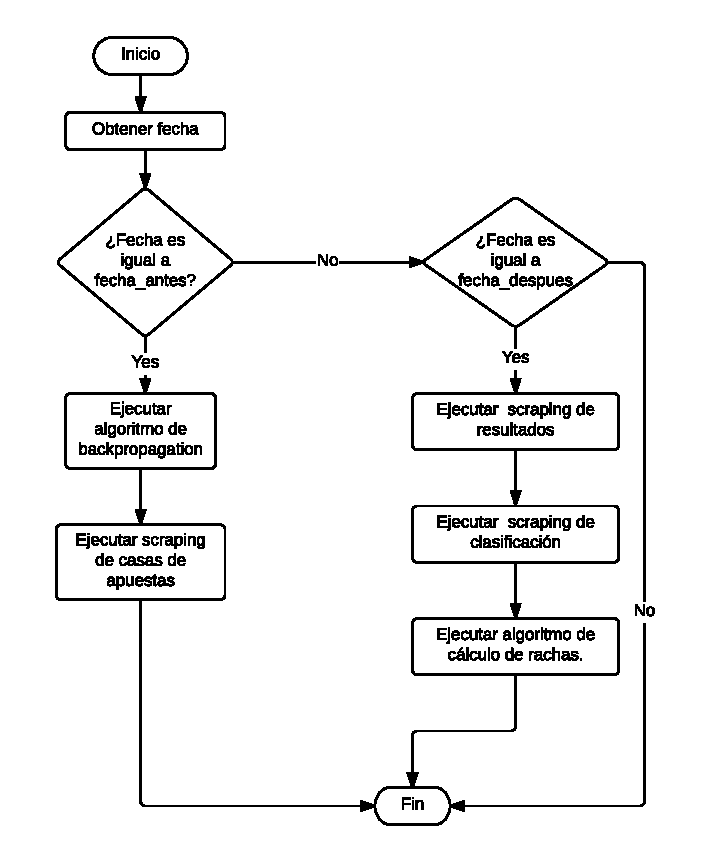
\includegraphics[width=.9\textwidth]{/img/Diagrama_flujo}
\caption{Diagrama de flujo}
\label{fig:DiagFluj}
\end{figure}

\section{Diseño arquitectónico}



\apendice{Documentación técnica de programación}

\section{Introducción}

\section{Estructura de directorios}

\section{Manual del programador}

\section{Compilación, instalación y ejecución del proyecto}

\section{Pruebas del sistema}

\apendice{Documentación de usuario}

\section{Introducción}
En este apéndice vamos a ver como instalar y realizar todas las acciones necesarias para poder ejecutar el proyecto finalmente.

\section{Requisitos de usuarios}
El objetivo de esta sección es indicar aquellos requisitos necesarios para que el usuario pueda utilizar el proyecto.

\subsection{Reguisitos software}
Es necesario tener instalado el gestor de máquinas virtuales Oracle VM Virtual Box. Este gestor puede ser utilizado prácticamente en cualquier sistema operativo, soportando la mayoría de sistemas Windows, Linux, Mac OS X y Solaris. Dado que la máquina es de 64 bits, en ocasiones nos encontramos con que Virtual Box no nos permite crearla, por ello es necesario tener activadas las opciones de virtualización desde la BIOS.

\subsection{Requisitos hardware}
En lo concerniente al hardware necesitamos un sistema que pueda correr sin problemas la máquina virtual. Como requisito mínimo es necesario un sistema cuya memoria RAM disponible para la máquina sea de 512 MB de RAM. En cuanto al espacio libre de disco es necesario al menos 20 GB. El procesador debe ser un x86, cualquier Intel o AMD reciente debe valer\cite{requeriments_VirtualBox}.


\section{Instalación}
Se va a proporcionar un disco que contiene la máquina en el formato \textit{Open Virtualization Format} <<OVF>>, que es un servicio virtualizado de la máquina virtual. En Oracle VM VirtualBox en la parte superior pulsamos \textit{Archivo} e \textit{Importar servicio virtualizado} como vemos en la figura \ref{fig:SerVir}, se abrirá una ventana donde debemos seleccionar la ubicación del servicio virtualizado. Automáticamente se pasará a una ventana cn las preferencias de la máquina por defecto como podemos ver en la figura \ref{fig:NueMaqVir}, y pulsamos \textit{Importar}. Por defecto tenemos 1 GB de RAM, que resulta suficiente para que funcione la máquina, si aumentamos la RAM veremos como aumenta la fluidez del servicio virtualizado.

\begin{figure}
\centering
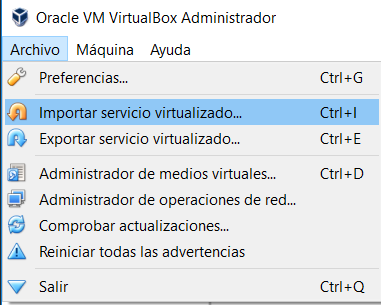
\includegraphics[width=.9\textwidth]{img/instalacion_user_servicio}
\caption{Importación de servicio virtual.}
\label{fig:SerVir}
\end{figure}

\begin{figure}
\centering
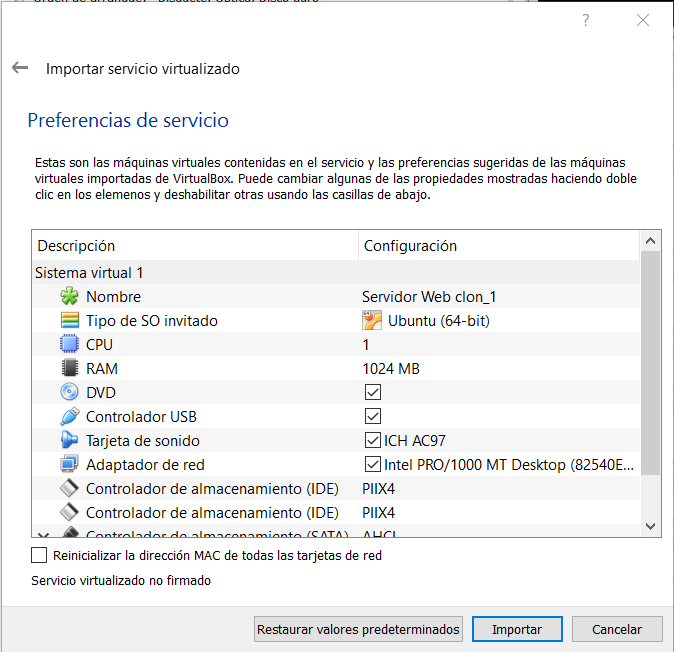
\includegraphics[width=.9\textwidth]{img/instalacion_user}
\caption{Preferencias del servicio virtual.}
\label{fig:NueMaqVir}
\end{figure}

Una vez iniciado es tan sencillo como abrir el Mozilla Firefox, cuyo icono encontramos a la izquierda en la barra de navegación de Ubuntu. Automáticamente debería abrirse en la página de inicio de nuestro sitio web, encaso de que no lo haga tecleamos en la barra de búsqueda \url{http://localhsot/inicio}. Una vez ya dentro, podremos utilizar el sitio web destinado.

\section{Manual del usuario}
El uso por parte del usuario de la aplicación web es muy sencilla, ya que las ejecuciones de los algoritmos están programadas por lo que no requiere intervención del usuario. El usuario se limita a observar los datos proporcionados por la interfaz, la interfaz es de sencillo uso y a continuación vamos a ver como utilizarla.

En la parte superior nos encontramos con una menú donde son 4 las opciones, como podemos observar en esta imagen\ref{fig:MenuDru}, y que vamos a describir brevemente:
\begin{figure}
\centering

\includegraphics[width=.9\textwidth]{img/drupal_menu}
\caption{Menú con el que puede interactuar el usuario.}
\label{fig:MenuDru}
\end{figure}

\begin{itemize}
\item \textbf{Inicio: } En esta opción nos encontramos con una breve descripción del proyecto y de las herramientas utilizadas.
\item \textbf{Informe General: } En este caso podemos observar del beneficio o pérdida obtenido en cada jornada y el balance global.
\item \textbf{Informe Jornada: } Si accedemos a través del menú podemos observar lo obtenido en una única jornada.
\item \textbf{Informe Pronóstico: } Nos proporciona los resultados que se esperan y las cuotas de las casas de apuestas.
\end{itemize}

Como podemos observar en la imagen, en esta primera página nos encontramos con la descripción del proyecto\ref{fig:IniDruUser}.

\begin{figure}
\centering
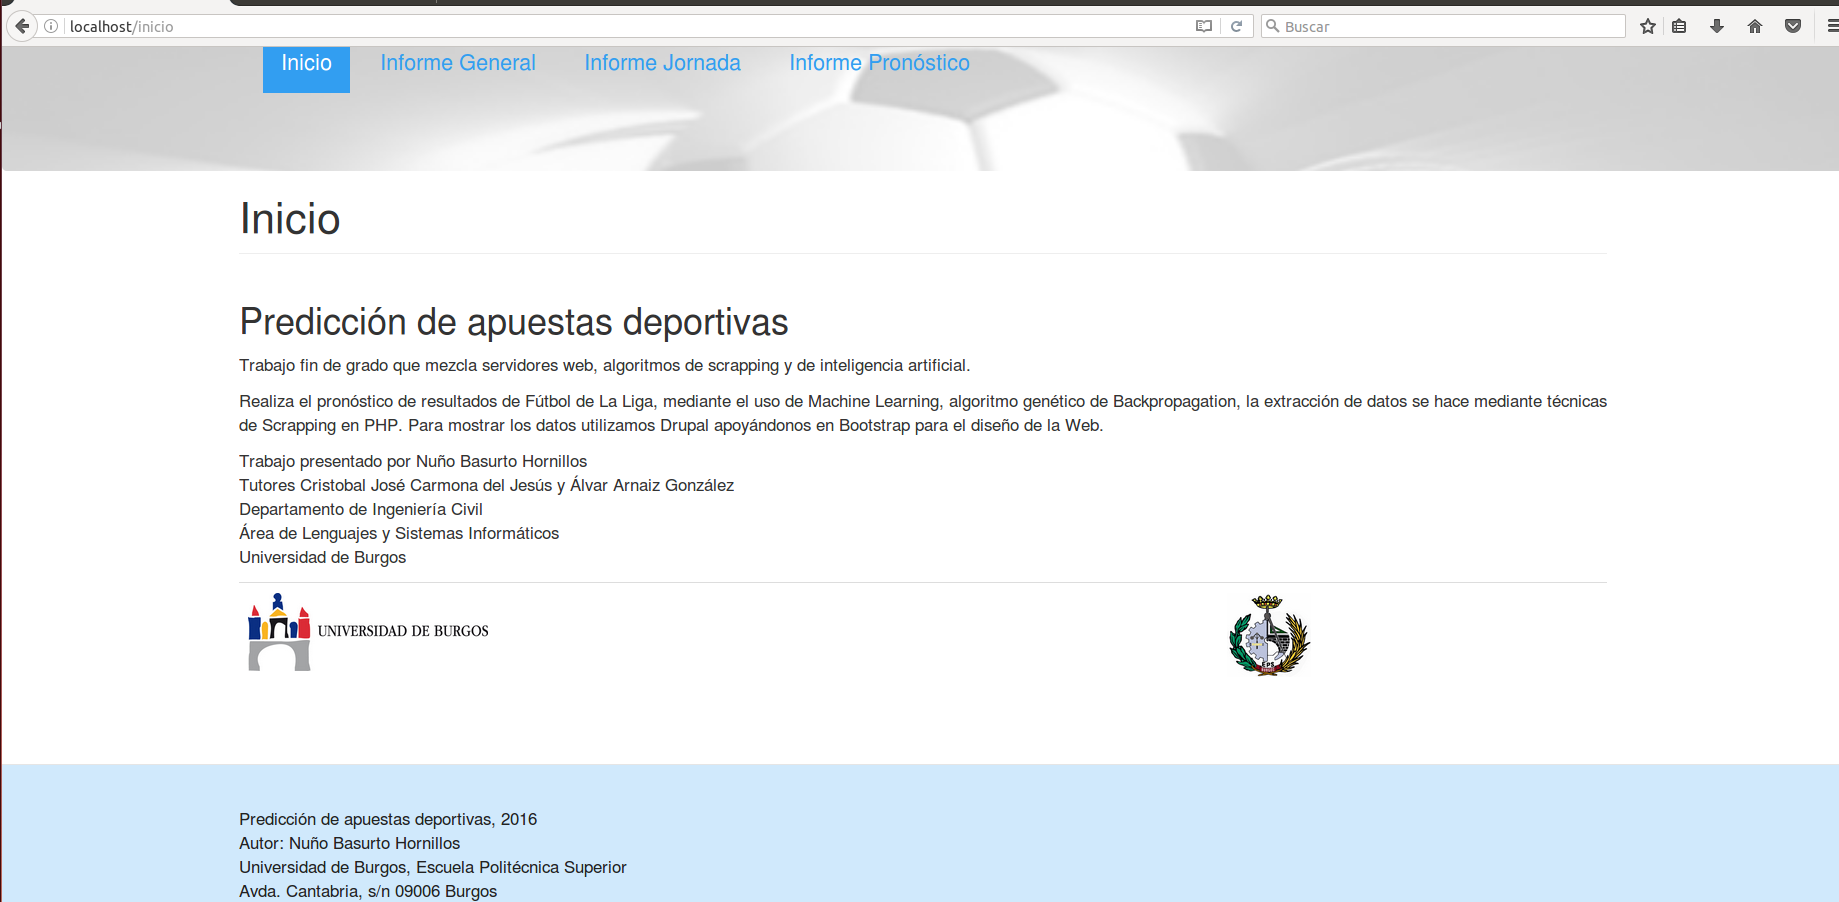
\includegraphics[width=.9\textwidth]{img/drupal_inicio_usuario}
\caption{Vista del usuario de Inicio.}
\label{fig:IniDruUser}
\end{figure}

En la ventana de informe general \ref{fig:InfGenDruUser}, podemos observar  una tabla con el balance de cada una de las jornadas, en cada una de las casas de apuestas, pulsando en la jornada accedemos a los partidos de la jornada más detalladamente, lo cuadros en verde son aquellos en los que se ha obtenido un balance positivo, en cambio encontramos en amarillo donde se pierde el dinero. Recordar que este es un balance por euro apostado. Por ejemplo en la jornada 14 observamos en la casa BET365 1.45 , entonces si apostásemos 10 en total (1 por partido) acabaríamos el día con 11.45, el 1.45 es el beneficio. En cambio en la jornada 15 en la misma casa de apuestas observamos -2.60, en este caso acabaríamos la jornada con 8.4, perdiendo dicho dinero.

\begin{figure}
\centering
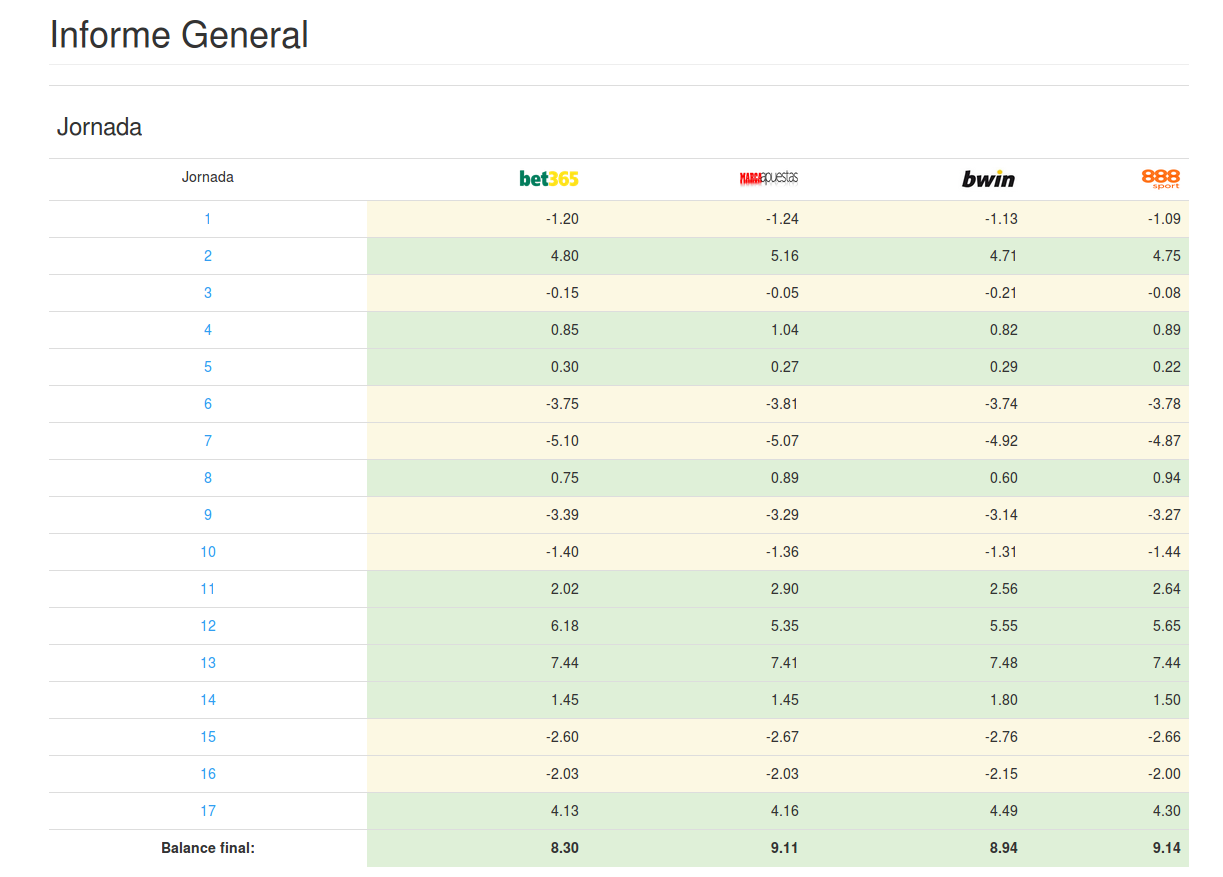
\includegraphics[width=.9\textwidth]{img/drupal_inf_general_usuario}
\caption{Vista del usuario del Informe de la Jornada.}
\label{fig:InfGenDruUser}
\end{figure}

A la ventana de Informe Jornada tenemos dos maneras de acceder, a través del menú donde observaremos el informe de la última jornada, o bien a través de los hipervínculos que encontramos en el Informe General, donde podemos acceder al resto de jornadas.
Podemos ves en negrita aquellos pronósticos que se han acertado, a su ves las casas de apuestas nos muestran lo predecido, mientras que aquellos partidos errados aparecen con -1 ya que el euro apostado en el partido se ha perdido. En la parte de abajo podemos observar el balance que veremos en amarillo si es negativo y en verde si es positivo.

En la imagen \ref{fig:InfJorDruUser}, observamos como la url es limpia por lo que nos muestra la última jornada a la que se ha accedido por el menú superior, en cambio si se ha accedido por el informe general veremos la imagen \ref{fig:InfJorDruUser2} con la URL diferente.

\begin{figure}
\centering
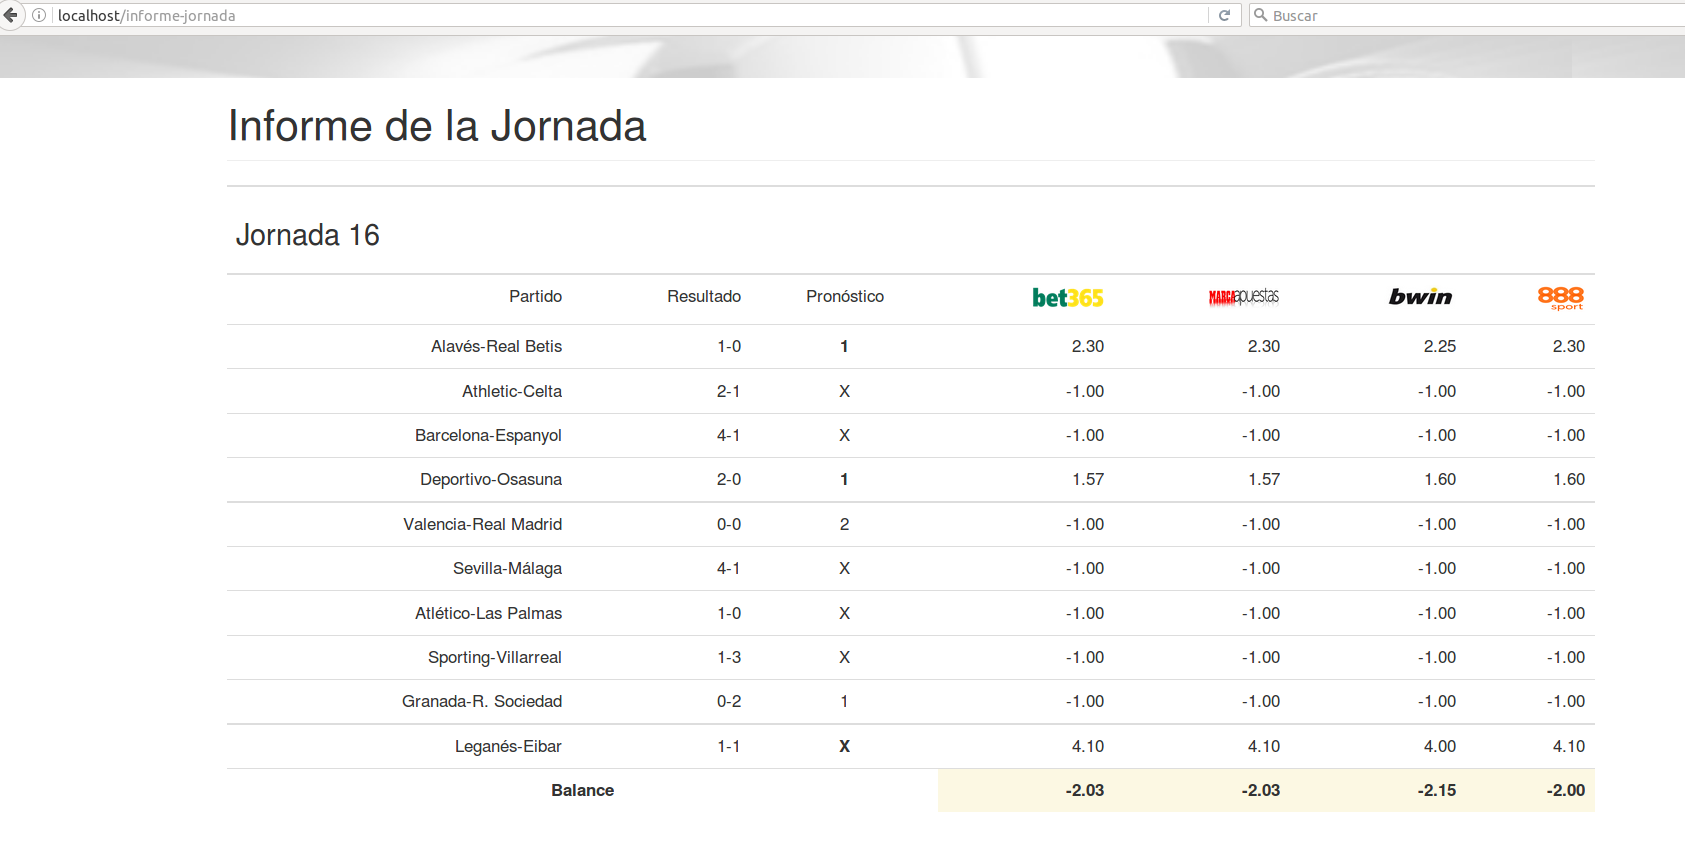
\includegraphics[width=.9\textwidth]{img/drupal_inf_jornada_usuario}
\caption{Vista del usuario del Informe Jornada.}
\label{fig:InfJorDruUser}
\end{figure}
\begin{figure}
\centering
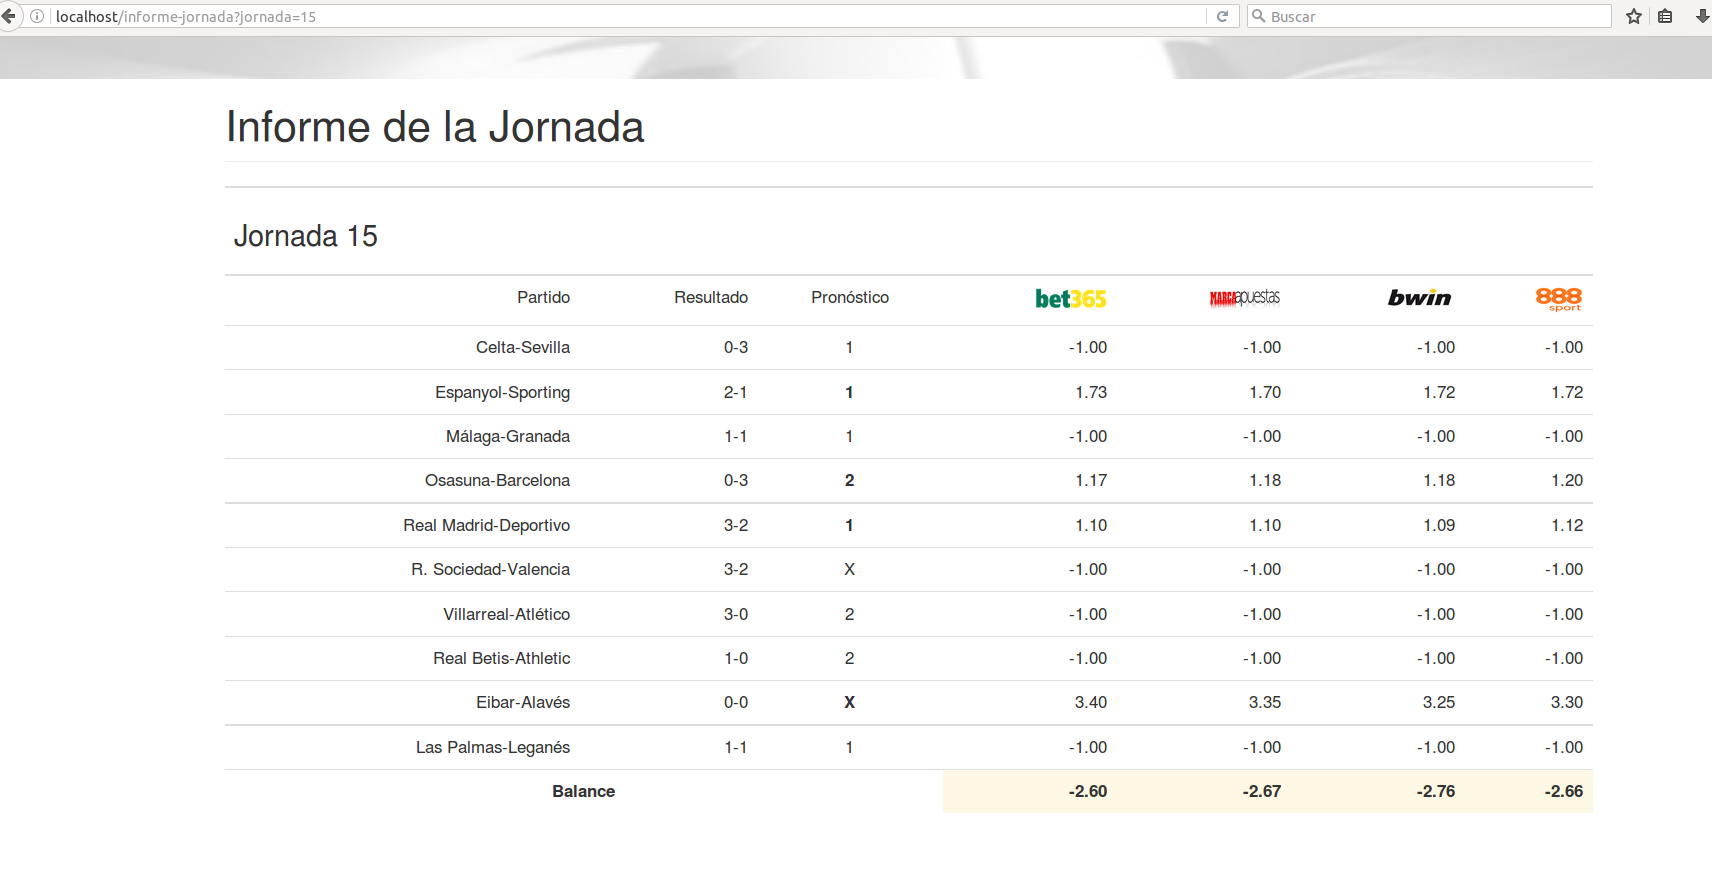
\includegraphics[width=.9\textwidth]{img/drupal_inf_jornada_usuario2}
\caption{Vista del usuario del Informe de la Jornada con la URL diferente.}
\label{fig:InfJor2DruUser}
\end{figure}

En el informe del pronóstico\ref{fig:InfProDruUser}, podemos observar todas las cuotas de los partidos para el pronóstico realizado. Y las ganancias potenciales que tenemos una vez finalizada la jornada se realizará el recuento y esta jornada pasará al informe de la jornada, poniendo aquí los partidos de la nueva jornada a la espera del pronóstico y de las cuotas de las casas de apuestas.

\begin{figure}
\centering
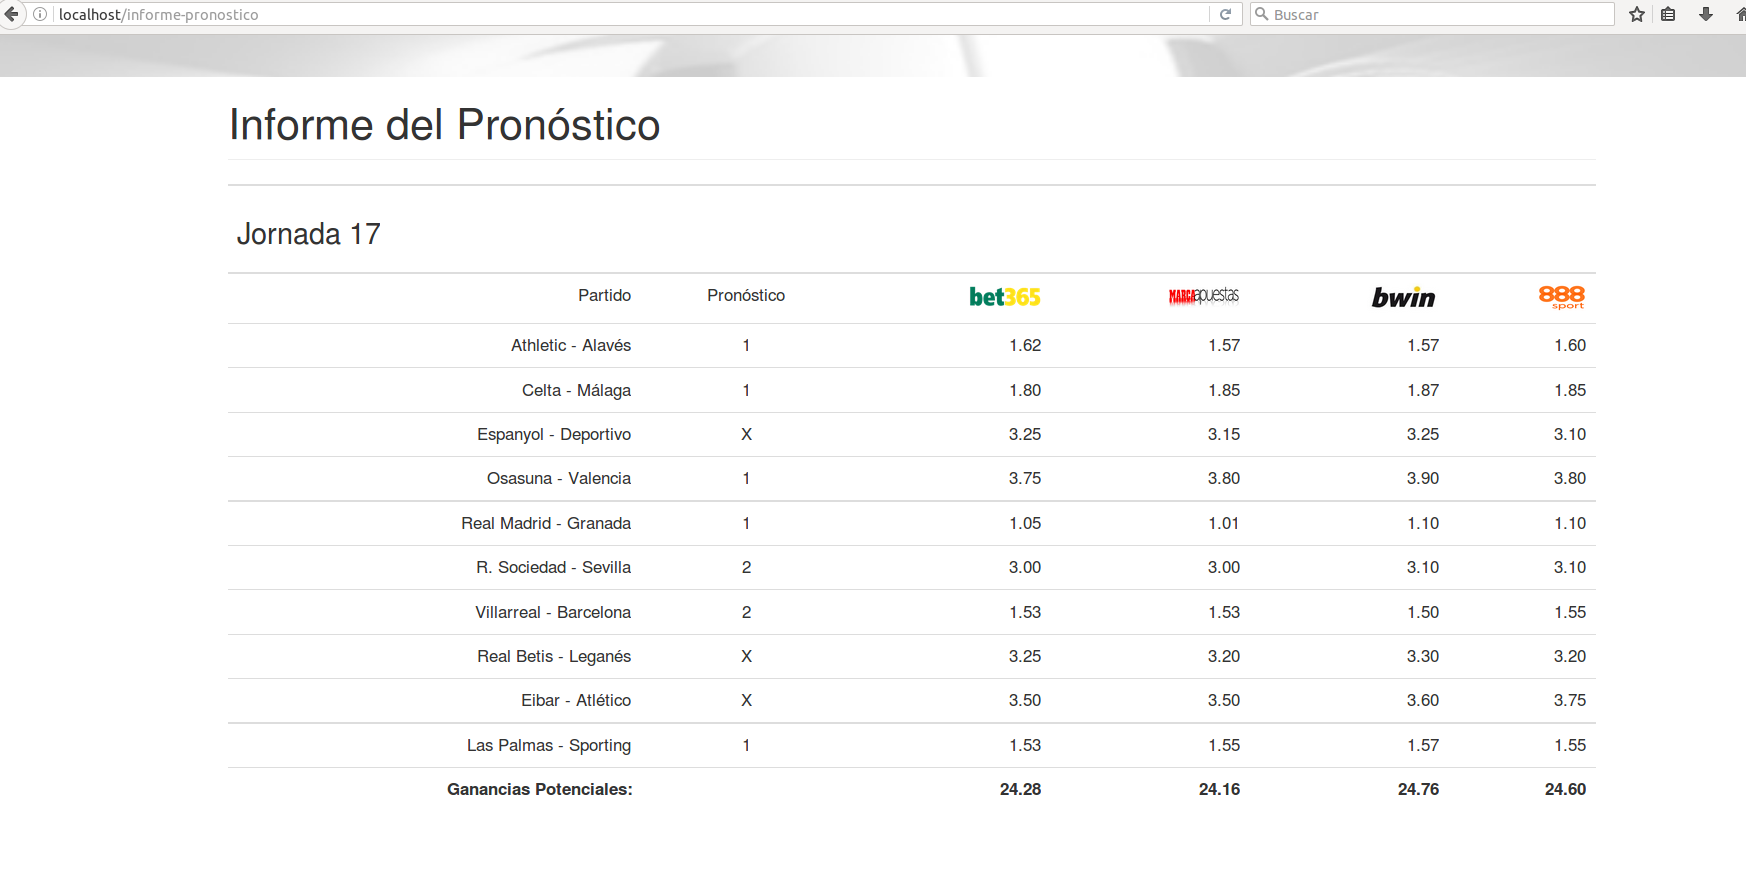
\includegraphics[width=.9\textwidth]{img/drupal_inf_pronostico_usuario}
\caption{Vista del usuario del Informe del pronóstico.}
\label{fig:InfProDruUser}
\end{figure}


\bibliographystyle{plain}
\bibliography{bibliografiaAnexos}

\end{document}